% ! TeX program = pdflatex

\documentclass{article}

\usepackage[a4paper, margin = 1in]{geometry}
\usepackage{listings}
\usepackage{color}
\usepackage{graphicx}
\usepackage{tikz}
\usepackage[maxbibnames=10]{biblatex} 
\addbibresource{references.bib}

\linespread{1.2}

\definecolor{mygreen}{rgb}{0,0.6,0}
\definecolor{mymauve}{rgb}{0.58,0,0.82}

\lstset{
	commentstyle=\color{mygreen},
	keywordstyle=\color{blue},
	stringstyle=\color{mymauve},
	identifierstyle=\color{cyan}
}

\newcommand{\code}[1]{\texttt{#1}}

\title
{
	CS420 Compiler Design\\
	Report for the Term Project: Internal Data Structure\\
	${}$\\
	Team 12
}

\author
{
	Jaeseong Choe\\
	Undergraduate\\
	Department of Physics, KAIST
	\and
	Kee Tack Kim\\
	Undergraduate\\
	Department of Mathematics, KAIST
	\and
	Taeyoung Kim\\
	Undergraduate\\
	School of Computing, KAIST
	\and
	Youngrae Kim\\
	Undergraduate\\
	School of Computing, KAIST
	\and
	Seokbin Lee\\
	Undergraduate\\
	School of Computing, KAIST
}

\begin{document}
	\maketitle
	
	\section{Token}
	
	The PLY library consist of two \code{.py} files. \code{lex.py} for lexical analyzer generator and \code{yacc.py} for syntax analyzer generator, respectively. In the \code{lex.py} file, there is a special class for tokenization phase called \code{LexToken}. The class \code{LexToken} has four attributes:
	
	\begin{itemize}
		\item \code{self.type}
		
		\code{self.type} field represent the type of each token. For example, lexime \code{1234} has the token type \code{ICONST} after it tokenized.

		\item \code{self.value}
		
		\code{self.value} field represent the original string of each token. For example, lexime \code{1234} has the value \code{`1234'} after it tokenized.

		\item \code{self.linno}
		
		\code{self.lino} field represent the line number of each lexime in the source file.

		\item \code{self.lexpos}
		
		\code{self.lexpos} field represent the position of first charactor of each lexime relative to the start of source file.
	\end{itemize}
	
	Figure \ref{fig: tokenization} shows that how the tokenization phase works. If the lexical analyzer meet \code{var = 1234;} at line 10 of source file, then it produces the tokens like \code{\code{(ID, `var', 10, 53)}}, \code{(ASSIGN, `=', 10, 57)}, \code{(ICONST, `1234', 10, 59)}, and \code{(COLON, `:', 10, 63)} with predefined matching rules for each lexime.
	
	\begin{figure}[ht]
		\centering
		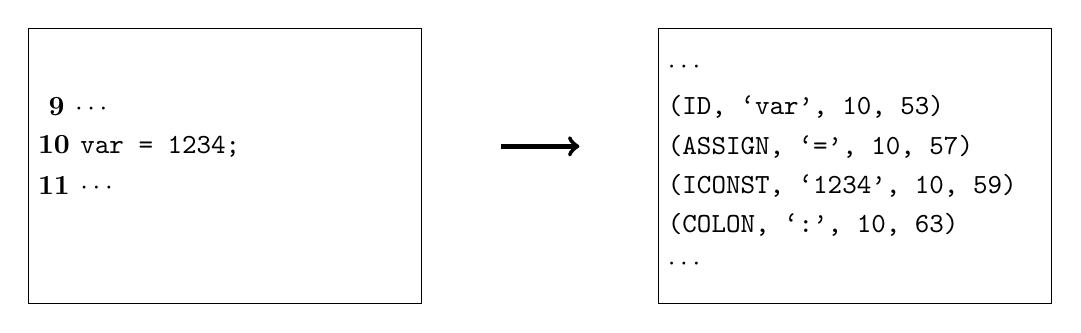
\begin{tikzpicture}
			\draw (0,3.5) rectangle (5,0);
			\draw (0,2.5) node[anchor=west] {\textbf{ 9 }\code{$\cdots$}};
			\draw (0,2.0) node[anchor=west] {\textbf{10 }\code{var = 1234;}};
			\draw (0,1.5) node[anchor=west] {\textbf{11 }\code{$\cdots$}};
			
			\draw[->, ultra thick] (6,2) -- (7,2);
			
			\draw (8,3.5) rectangle (13, 0);
			\draw (8,3.0) node[anchor=west] {\code{$\cdots$}};
			\draw (8,2.5) node[anchor=west] {\code{(ID, `var', 10, 53)}};
			\draw (8,2.0) node[anchor=west] {\code{(ASSIGN, `=', 10, 57)}};
			\draw (8,1.5) node[anchor=west] {\code{(ICONST, `1234', 10, 59)}};
			\draw (8,1.0) node[anchor=west] {\code{(COLON, `:', 10, 63)}};
			\draw (8,0.5) node[anchor=west] {\code{$\cdots$}};
		\end{tikzpicture}
		\caption{Tokenization.}
		\label{fig: tokenization}
	\end{figure}
	
	\section{Abstract syntax tree}
	
	In order to implement the abstract syntax tree (AST), we implement the class \code{Node}. The class \code{Node} has two attribute:
	
	\begin{itemize}
		\item \code{self.data}
		
		\code{self.data} is a field to represent general data contained in that node. The type of data can be anything by the beauty of Python!

		\item \code{self.children}
		
		\code{self.children} is a field that represent the children of that node. The type of it is a list.
	\end{itemize}
	
	Figure \ref{fig: class node} shows that the graphical explanation of the class \code{Node}.
	
	\begin{figure}[ht]
		\centering
		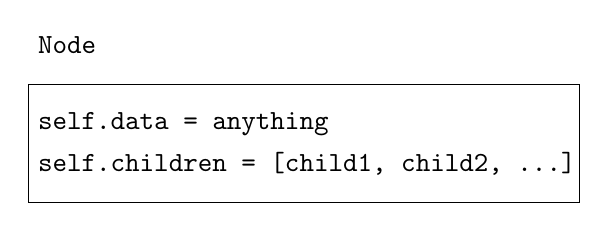
\begin{tikzpicture}
			\draw (0,2.0) node[anchor=west] {\code{Node}};
			\draw (0,1.5) rectangle (7,0);
			\draw (0,1.0) node[anchor=west] {\code{self.data = anything}};
			\draw (0,0.5) node[anchor=west] {\code{self.children = [child1, child2, \dots]}};
		\end{tikzpicture}
		\caption{Class \code{Node}.}
		\label{fig: class node}
	\end{figure}
	
	\section{Symbol table}
	Our symbol table structure has the hierarchy as shown in Figure \ref{fig: hierarchy of symbol table} by its scope (or block). In order to implement this hierarchy, we define the two classes \code{SymTabBlock} and \code{SymTab}. The class \code{SymTabBlock} represents a symbol table for certain block, and \code{SymTab} represents and manages a overall hierarchy of these blockwise symbol tables.
	
	\begin{figure}[ht]
		\centering
		\includegraphics[width=0.55\textwidth]{"../img/symbol table hierarchy".png}
		\caption{The hierarchy of symbol table. \cite{Aho:2006:CPT:1177220}}
		\label{fig: hierarchy of symbol table}
	\end{figure}
	
	Furthermore, there is one another class for collecting the data about certain symbol (or identifier) called \code{SymTabEntry}. The class \code{SymTabEntry} has three attributes:
	
	\begin{itemize}
		\item \code{self.id}
		
		\code{self.id} field represents the identifier as a string.
		
		\item \code{self.type}
		
		\code{self.type} field represents the type of that identifier. For example, if the identifier \code{var} declared in source file with the type \code{int}, then \code{self.type} of \code{SymTabEntry} for this identifier is \code{INT}.
		
		\item \code{self.assigned}
		
		\code{self.assigned} field represents the weather some value was assigned to that identifier or not by boolean (\code{True} or \code{False}).
	\end{itemize}
	
	\code{SymTabBlock} is a symbol table of each block. The class \code{SymTabBlock} has three attributes:
	
	\begin{itemize}
		\item \code{self.prev}
		
		\code{self.prev} field represents the symbol table of the direct outer block of current block. For example, in the case of Figure \ref{fig: hierarchy of symbol table}, \code{self.prev} of $B_1$ pointing to $B_0$.
		
		\item \code{self.nexts}
		
		\code{self.nexts} field represent the list of symbol tables for the direct inner blocks of current block. For example, in the case of Figure \ref{fig: hierarchy of symbol table}, \code{self.nexts} of $B_1$ is a list \code{[$B_2$, \dots]}.
		
		\item \code{self.table}
		
		\code{self.table} is an actual table to save the information about each symbols. It is a dictionary object which is a builtin hash table object in Python. Hence, it corresponds to table in the right side of each labels in Figure \ref{fig: hierarchy of symbol table}.
	\end{itemize}
	
	\code{SymTab} is a management system for overall collection of \code{SymTabBlock}. The class \code{SymTab} has one attribute and five methods:
	
	\begin{itemize}
		\item \code{self.cur}
		
		\code{self.cur} pointing to the current symbol table.
		
		\item \code{insert\_block\_table(self, block\_table)}
		
		\code{insert\_block\_table} method provides feature that insert new symbol table into the management system. It appends the \code{block\_table} into the list \code{self.nexts} of the current symbol table. Then, it changes \code{self.cur} to \code{block\_table}.
		
		\item \code{remove\_block\_table(self)}
		
		\code{remove\_block\_table} method provides feature that remove the current symbol table. It pops the current symbol table from the list \code{self.nexts} of symbol table for direct outer block. Then, it changes \code{self.cur} to symbol table for direct outer block. 
		
		\item \code{insert(self, symbol)}
		
		\code{insert} method provides a feature that register the information of new symbol into current symbol table. The input parameter \code{symbol} is a \code{SymTabEntry} object. \code{insert} method check that there already exist a symbol with same identifier with the input parameter \code{symbol}. If there is no such a symbol, then \code{insert} registers the \code{symbol} into current symbol table with setting the hash key as its identifier \code{symbol.id}. If there is such a symbol, \code{insert} produces an error \code{DupDeclError}.
		
		\item \code{remove(self, id)}
		
		\code{remove} method provides a feature that deregister the information about identifier \code{id} from the current symbol table. \code{remove} check weather there exist the information about that identifier. If there is such information, then it removes the hash information of that identifier. If there no such information, then it produces an error \code{UndefIdError}.
		
		\item \code{get(self, id)}
		
		\code{get} method provides a feature that searching the information about identifier \code{id}. \code{get} searches the information with the manner of starting from current symbol table to outer symbol tables. If \code{get} succeed to find that information, then it returns that information as the form of \code{SymTabEntry}. If \code{get} failed to find that information, then it produces an error \code{UndefIdError}.
	\end{itemize}
	
	Figure \ref{fig: illustration of the hierarchy of symbol table classes} illustrates the hierarchy of symbol table. The outermost rectangle of blue color represents the symbol table management class \code{SymTab}. An arrow represents the \code{self.cur} attribute of \code{SymTab}. The rest rectangles of gray color represent the symbol tables class \code{SymTabBlock} for each blocks.
	
	\begin{figure}[ht]
		\centering
		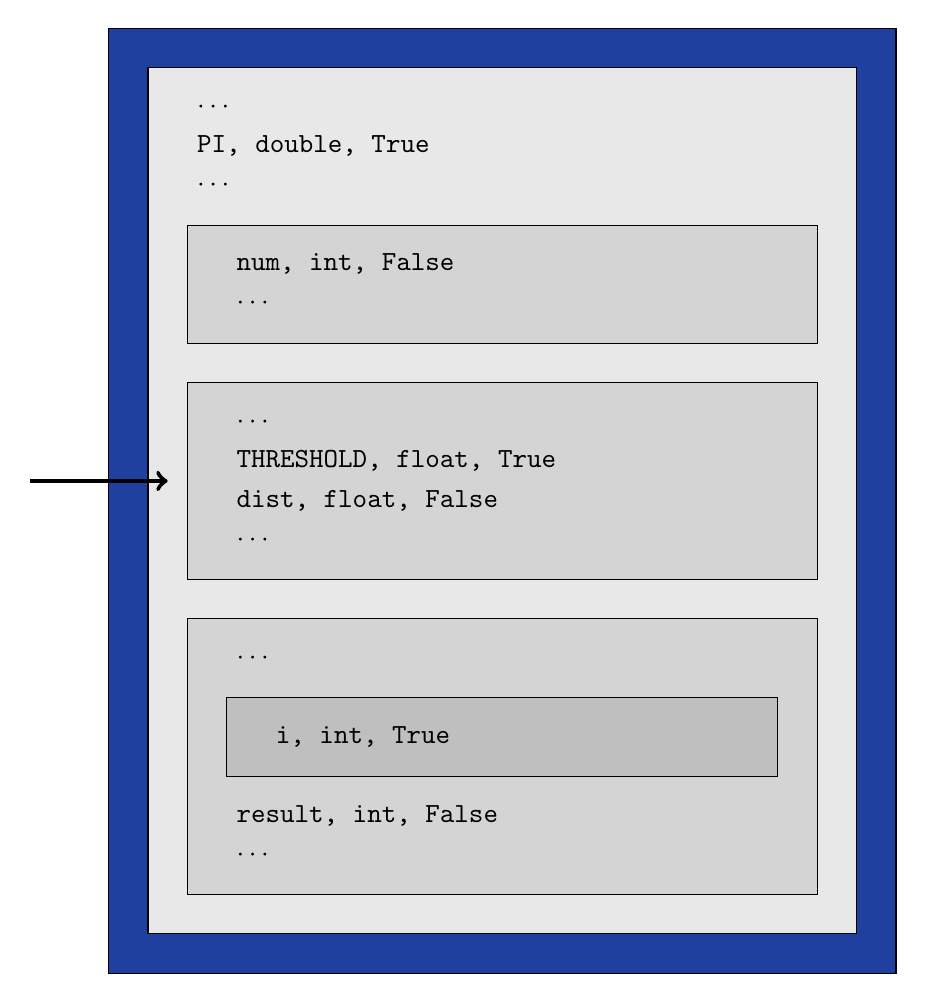
\begin{tikzpicture}
			\draw[fill={rgb:red,1;green,2;blue,5}] (0,0) rectangle (10, 12);
			
			\draw[fill={rgb:black,1;white,10}] (0.5,0.5) rectangle (9.5, 11.5);
			
			\draw[fill={rgb:black,1;white,5}] (1,1) rectangle (9, 4.5);
			\draw[fill={rgb:black,1;white,5}] (1,5) rectangle (9, 7.5);
			\draw[fill={rgb:black,1;white,5}] (1,8) rectangle (9, 9.5);
			
			\draw[fill={rgb:black,1;white,3}] (1.5,2.5) rectangle (8.5, 3.5);
			
			
			\draw (1,11) node[anchor=west] {\code{$\cdots$}};
			\draw (1,10.5) node[anchor=west] {\code{PI, double, True}};
			\draw (1,10) node[anchor=west] {\code{$\cdots$}};
			
			\draw (1.5,9) node[anchor=west] {\code{num, int, False}};
			\draw (1.5,8.5) node[anchor=west] {\code{$\cdots$}};
			
			\draw (1.5,7) node[anchor=west] {\code{$\cdots$}};
			\draw (1.5,6.5) node[anchor=west] {\code{THRESHOLD, float, True}};
			\draw (1.5,6) node[anchor=west] {\code{dist, float, False}};
			\draw (1.5,5.5) node[anchor=west] {\code{$\cdots$}};
			
			\draw (1.5,4) node[anchor=west] {\code{$\cdots$}};
			\draw (2,3) node[anchor=west] {\code{i, int, True}};
			\draw (1.5,2) node[anchor=west] {\code{result, int, False}};
			\draw (1.5,1.5) node[anchor=west] {\code{$\cdots$}};
			
			
			\draw[->, ultra thick] (-1,6.25) -- (0.75,6.25);
		\end{tikzpicture}
		\caption{Illustration of the hierarchy of symbol table classes.}
		\label{fig: illustration of the hierarchy of symbol table classes}
	\end{figure}
	
	\section{Intermediate code}
	We uses the three-address code format for the our internal intermediate code, i.e., our intermediate code is the form of
	\[ \code{x = y op z}. \]
	The detailed specification of intermediate code for each statement does not defined yet. However, we try to specifying it in the next week.
	
	\printbibliography
\end{document}